
\documentclass{article}

\usepackage{titlesec}
\newcommand{\sectionbreak}{\clearpage}

\usepackage{fancyhdr}
\pagestyle{fancy}
\lhead{Emanuel Casiano-Diaz}
\rhead{CSYS300: PoCS - Homework 05 - 10/05/2018}
\renewcommand{\headrulewidth}{0.4pt}
\renewcommand{\footrulewidth}{0.4pt}

\usepackage{amsmath}
\usepackage{amssymb}
\usepackage{bm}
\usepackage{pdfpages}

\usepackage{enumerate}% http://ctan.org/pkg/enumerate

\usepackage{hyperref}
\hypersetup{
    colorlinks=true,
    linkcolor=blue,
    filecolor=magenta,      
    urlcolor=cyan,
}

\usepackage{booktabs,float,siunitx}
%\usepackage[demo]{graphicx} % omit 'demo' option in real document

\begin{document}

\section{Exercise 1: Generalized entropy and diversity}

Strategy: Equate the corresponding information measure of text $T$ to that of text $T'$ and solve for the diversity, $D$. The probabilities will be given by $p_i = \frac{1}{D}$.

\subsection{a) Simpson Concentration}
\begin{align}
S[T] &= S[T'] \\
&= \sum_{j=1}^{D} p_j^2 \\
&= \sum_{j=1}^{D} (\frac{1}{D})^2 \\
&= (D) (\frac{1}{D^2}) \\
S[T] &= D^{-1} = \sum_{i=1}^{n} p_i^2 \\
\implies D &= \frac{1}{\sum_{i=1}^{n} p_i^2}
\end{align}

\subsection{b) Gini Index}
\begin{align}
G[T] &= G[T'] \\
&= 1 - \sum_{j=1}^{D} p_j^2 \\
G[T ] &= 1 - D^{-1} = 1 - \sum_{i=1}^{n} p_i^2 \\
\implies D &= \frac{1}{\sum_{i=1}^{n} p_i^2} 
\end{align}

The Simpson Concentration and Gini Concentration have the same diversity! 

\subsection{c) Shannon Entropy}
\begin{align}
H[T] &= H[T'] \\
&= - \sum_{j=1}^D p_j \ln p_j \\
&= - (D) (\frac{1}{D}) \ln (\frac{1}{D}) \\
&= -\ln(\frac{1}{D}) \\
H[T] &= \ln D = - \sum_{i=1}^{n} p_i \ln p_i \\
\implies D &= e^{-\sum p_i \ln p_i}
\end{align}

Note: In the line above, the lower and upper limits of the summation have been left out for esthetic reasons.

\subsection{d) Renyi Entropi}
\begin{align}
H_{q}^{(R)}[T] = H_{q}^{(R)}[T'] \\
&= \frac{1}{q-1} [-\ln \sum_{j=1}^D p_j^q] \\
&= \frac{1}{1-q}\ln [(D)(\frac{1}{D})^q] \\
&= \frac{1}{1-q} \ln [D^{1-q}] \\
H_q^{(R)} &= \ln D = \frac{1}{1-q} \ln \sum_{i=1}^{n} p_i^q \\
\implies D &= [\sum_{i=1}^n p_i^q]^{\frac{1}{1-q}}
\end{align}
\subsection{e) Generalized Tsallis Entropy}

\begin{align}
H_q^{(Ts)} [T] &= H_q^{(Ts)} [T'] \\
&= \frac{1}{q-1} - \frac{1}{q-1} [\ln \sum_{j=1}^D p_j^q]  \\
H_q^{(Ts)} [T] &= \frac{1}{q-1} + \ln D = \frac{1}{q-1} - \frac{1}{q-1} [\ln \sum_{i=1}^D p_i^q] \\
\implies \ln D &= - \frac{1}{q-1} [\ln \sum_{i=1}^D p_i^q] \\
\implies D &=  [\sum_{i=1}^n p_i^q]^{\frac{1}{1-q}}
\end{align}

The Renyi Entropy and Generalized Tsallis Entropy have the same diversity!

\subsection{f) The limiting case of $q \to 1$}

Here it will be shown that as $q\to1$, the diversity of the Renyi and Generalized Tsallis Entropy becomes the diversity of the Shannon Entropy. For simplicity (hopefully), the limit will be evaluated for $\ln D$ instead, then exponentiated at the end.

\begin{align}
\lim_{q\to1} \ln D = \lim_{q \to 1} \frac{\ln[\sum_{i=1}^n p_i^q]}{1-q} = \frac{0}{0}
\end{align}

Recall that the probabilities are normalized. In other words, $\sum_{i} = p_i = 1$ and $\ln{1} = 0$. This is the reason why the indeterminate form $\frac{0}{0}$ is obtained. Applying L'Hopital's Rule once will get rid of this issue:

\begin{align}
\lim_{q\to1} \ln D &=  -\lim_{q\to1} \frac{d}{dq} [\sum_i p_i^q] ; \text{ via L'Hopital} \\
\end{align}
\\
Now, there's three rules that will be convenient to recall: \\
\\
1. Differential operators can be interchanged with summations \\
2. $\frac{d}{dx} \ln f(x) = \frac{f'(x)}{f(x)}$ \\
3. $\frac{d}{dx} a^x = a^x \ln a$, where $a>0$ and $a\neq1$ \\

Thus, applying these to the right hand side (RHS) of the above equation, the limit becomes:

\begin{align}
\lim_{q\to1} \ln D &= -\lim_{q\to1} [\frac{\sum_i p_i^q \ln p_i}{\sum_i p_i^q}]
 \end{align}

Applying the normalization condition to the denominator in the RHS:

\begin{align}
\lim_{q\to1} \ln D &= -\lim_{q\to1}  [\sum_i p_i^q \ln p_i] = - [\sum_i p_i \ln p_i] \\
\implies \lim_{q\to1} D &= e^{- \sum_i p_i \ln p_i}
\end{align}

$\therefore$ In the limit $q\to1$, the Diversity of the Renyi and Generalized Tsallis Entropies becomes the Shannon Entropy Diversity!

\section{Exercise 2: Mandelbrotian derivation of Zipf's Law}

Want: The set of probabilities $p_i$ that minimize $\Psi$. Thus, need to solve the following equation for $p_i$:

\begin{align}
\frac{d\Psi}{dp_i} &= \frac{dF}{dp_i} + \lambda \frac{dG}{dp_i} = 0
\end{align}

NOTE: The derivatives are rather extensive to type in LaTeX in excruciating detail. As such, only the key ideas behind it will be discussed here. To see my full derivation, please follow this link: \url{https://github.com/ecasiano/PrinciplesOfComplexSystems/blob/master/HW05/Q02/CSYS300_%20HW05.pdf} \\

The function $F(\lbrace p_i \rbrace)$ is the "Cost over Information" function and is defined as:

\begin{align}
F(\lbrace p_i \rbrace) = \frac{C}{H}
\end{align}

where $C = \sum_{i=1}^{n} p_i \ln(i+a)$ and $H = -g \sum_{i=1}^{n} p_i \ln p_i$. The derivative of $F$ respect to $p_i$ becomes:

\begin{align}
\frac{dF}{dp_i} &= -\frac{1}{g} [\frac{\sum_i \ln (i+a)}{\sum_i p_i \ln p_i} - \frac{(\sum_i p_i \ln(i+a))(\sum_i(\ln p_i + 1))}{(\sum_i p_i \ln p_i)^2}]
\end{align}

Which, using the definition for the cost and information functions, can be rewritten as:

\begin{align}
\frac{dF}{dp_i} &= \frac{\sum_i \ln(i+a)}{H} + \frac{gC\sum_i(\ln p_i + 1)}{H^2}
\end{align}

The function $G(\{ p_i \})$ is known as the "constraint equation" and, for this case, is defined as:

\begin{align}
G(\{ p_i \}) &= -1 + \sum_i p_i = 0
\end{align}

i.e, G is the normalization condition for the probabilities. Taking the derivative of $G$ with respect to $p_i$, it is seen that:

\begin{align}
\frac{dG}{dp_i} &= \sum_{i} 
\end{align}

Don't worry, the summand is not missing, it is just 1 :) \\

Substituting the derivatives of $F$ and $G$ into $\frac{d\Psi}{dp_i}$:

\begin{align}
\frac{d\Psi}{dp_i} &= \frac{\sum_i \ln(i+a)}{H} + \frac{gC\sum_i(\ln p_i + 1)}{H^2} + \lambda \sum_i = 0
\end{align}

The above expression can be all written as a single sum, instead of four:

\begin{align}
\sum_{i}[\frac{1}{H} \ln(i+a) + \frac{gC}{H^2} \ln p_i + \frac{gC}{H^2} + \lambda] = 0
\end{align}

The summand must then be zero. Setting the summand to zero and solving for $\ln p_i$:

\begin{align}
\ln p_i &= -1-\frac{\lambda H^2}{gC} + \ln(i+a)^{-H/gC}
\end{align}

Exponentiating on both sides of the equation:

\begin{align}
p_i &= e^{-1-\frac{\lambda H^2}{gC}}(i+a)^{-H/gC}
\end{align}

Thus, the probabilities follow a power-law scaling $p_i \propto (i+a)^{-H/gC}$. Nevertheless, an exact solution can be obtained for $p_i$ by determining the value of the pre-factor. Substituting the expression for $\ln p_i$ into the definition of $H$ (but not $p_i$), it can be seen that:

\begin{align}
H = g + \frac{\lambda H^2}{C} + H
\end{align}

Solving for $\lambda$:

\begin{align}
\lambda &= -\frac{gC}{H^2}
\end{align}

Substituting this expression for $\lambda$ into the exponent of the pre-factor of $p_i$, the terms in the exponent cancel out to zero and, thus, the pre-factor becomes unity. Therefore, the exact solution for $p_i$ is:

\begin{align}
p_i &= (i+a)^{-H/gC}
\end{align}

$\therefore$ The probabilities follow an Inverse Power-Law Scaling of $p_i = (i+a)^{-\alpha}$, where $\alpha = \frac{H}{gC}$.

\section{Exercise 3: Testing out the previous result}

The code developed to solve this exercise can be found here: \url{https://github.com/ecasiano/PrinciplesOfComplexSystems/blob/master/HW05/Q03/zipfarama.py} 

\subsection{a)}
In the previous problem, it was obtained that:

\begin{align}
p_i &= (i+a)^{-\alpha}
\end{align}

In the case that $a=1$ and $n\to\infty$, an estimate of the scaling exponent $\alpha$ can be obtained computationally. First of all, recall, the normalization condition on the probabilities:

\begin{align}
\sum_{i=1}^{n} (i+a)^{-\alpha} &= 1 
\end{align}

Below, the algorithm developed is illustrated. \\

\textbf{Algorithm:} \\
.---------------------------------.\\
1. Initialize random value of $\alpha$ \\
2. Set desired tolerance \\
3. Calculate the error: $| \sum_i^{n} (i+a)^{\alpha} - 1 | $ \\
4. While error $>$ tolerance: \\
	\indent{-If $\sum_i^{n} (i+a)^{\alpha} < 1$}, decrease $\alpha$ \\
	\indent{-else, increase $\alpha$} \\
	\indent{-Recalculate the error} \\
.---------------------------------.

Running the above routine for $n = 1,000,000$ words, the scaling exponent was estimated as $\alpha \approx 1.73$. The terminal output in Figure 1 shows all the iterations of the loop, with the corresponding value of $\alpha$ and the absolute error of the normalization.

\begin{figure}[h]
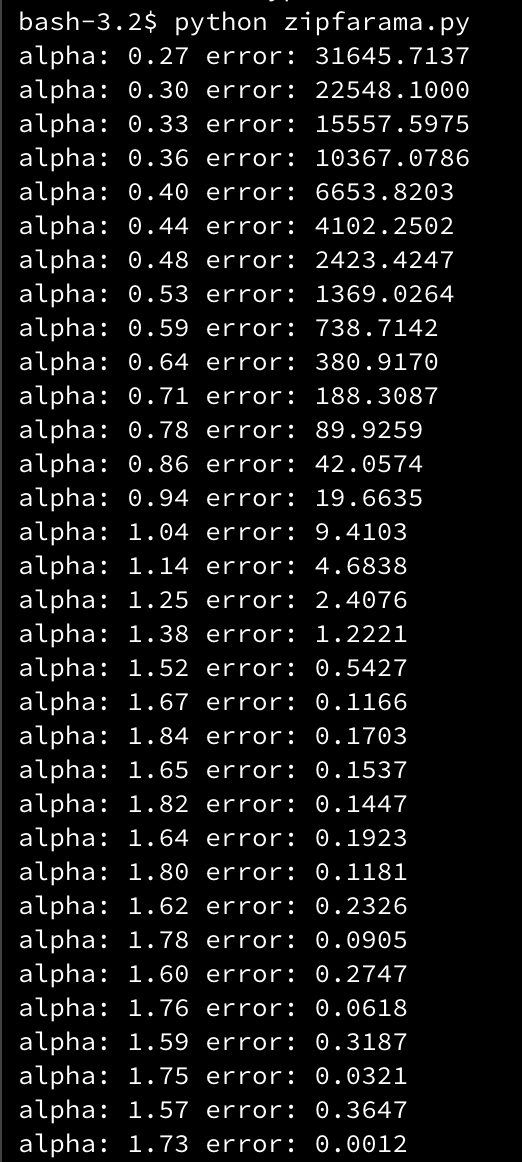
\includegraphics[height=15cm,width=15cm,keepaspectratio]{Q03/zipfaramaOutput.png}
\caption{Terminal output for the algorithm described to estimate the scaling exponent $\alpha$. For this run the number of words or elements in the summation has been set to $n = 1,000,000$ and $a = 1$. }
\label{fig:envelope}
\end{figure}

\begin{figure}[h]
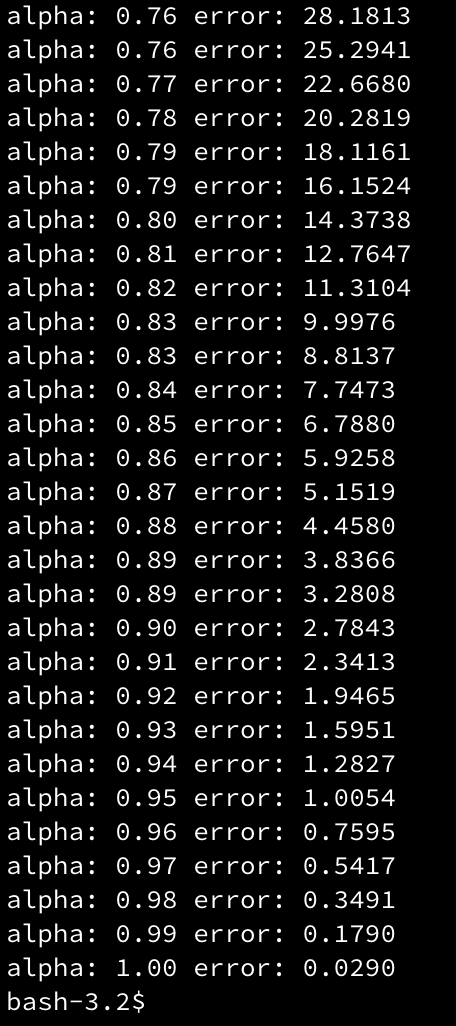
\includegraphics[height=15cm,width=15cm,keepaspectratio]{Q03/zipfaramaOutput_3b.png}
\caption{Terminal output for the algorithm described to estimate the scaling exponent $\alpha$. For this run the number of words or elements in the summation has been set to $n = 1,000,000$ and $a = \frac{e-n}{1-e}$. }
\label{fig:envelope}
\end{figure}

\subsection{b)}

Want: Estimate the value of $a$ that gives $\alpha = 1$ in terms of $n$ by approximating the summation of the normalization condition as an integral.\\
\\
The normalization condition can be approximated as an integral as:

\begin{align}
\sum_{i=1}^{n} (i+a)^{-\alpha} &= 1 \to \int_{1}^{n} (x+a)^{-\alpha} dx = 1
\end{align}

Setting $\alpha = 1$:

\begin{align}
\int_{1}^{n} \frac{1}{x+a} dx = 1
\end{align}

Using the substitution: $u = x + a$ and $du = dx$, the integral becomes:

\begin{align}
\int_{1+a}^{n+a} \frac{1}{u} du = 1
\end{align}

Note that the limits of integration have been replaced by $u(x=1)$ (lower limit) and $u(x=n)$ (upper limit). The definite integral becomes:

\begin{align}
\int_{1+a}^{n+a} \frac{1}{u} du &= \ln u |_{u=1+a}^{u=n+a} = \ln(\frac{n+a}{1+a}) = 1
\end{align} 

Exponentiating the last part of the line above:

\begin{align}
\frac{n+a}{1+a} = e
\end{align}

Solving for a:

\begin{align}
a = \frac{e-n}{1-e} 
\end{align}

In the limit of $n\to\infty$, $a\to\infty$ $\implies p_i \to 0$. In other words, the probabilities, which follow an inverse-power law will vanish. This makes sense, since it is expected that the probability associated with element $i$ will become increasingly small the larger the sample becomes. \\

The referenced code confirms the above result. Just substitute the parameter $a$ in the code by the derived expression and alpha will end up being $\alpha=1$ after a few iterations. See Figure 2.

\section{Exercise 4: Extrapolating a CCDF given it's fit}

The code used to generate the plot and estimates in this exercise is found here: \url{https://github.com/ecasiano/PrinciplesOfComplexSystems/blob/master/HW05/Q04/completeDist.py}

\subsection{a) and b)}

\begin{figure}[h!]
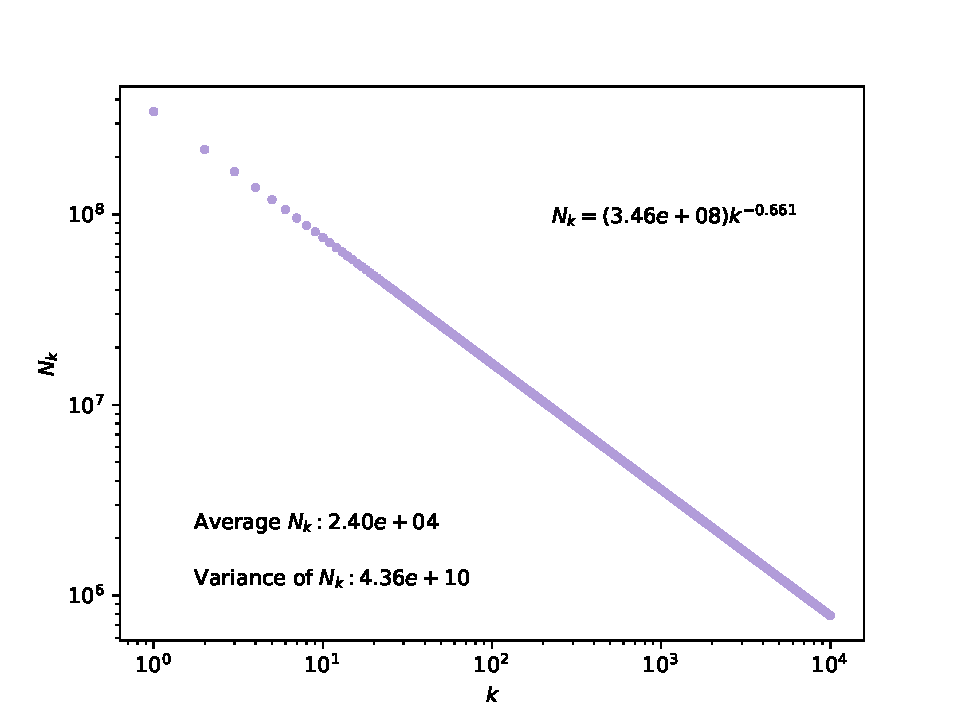
\includegraphics[width=\linewidth]{Q04/wordFrequencyCCDFLog_extrapolated.pdf}
\caption{Reconstructed distribution of group sizes $N_k$ as a function of $k$. $N_k$ represents the number of distinct words that show up with frequency $k$. This distribution was generated by extrapolating the given CCDF, which spans from $k=200$ to $k=10^7$, to the range $k:[1,199]$. NOTE: For ease of loading the image, only 5 orders of magnitude in $k$ have been plotted. Nevertheless, the distribution has been calculated for the full of range of frequencies, $k \in [10^0,10^7]$.}
\end{figure}

\subsection{c) Fraction of words that show up only once}

Define the total number of words, t, as:

\begin{align}
t = \sum_{\text{All }k} k N_k
\end{align}

The fraction of words that show up only once out of all the words, $N_1^{(g)}$ can be obtained by:

\begin{align}
N_1^{(g)} = \frac{N_1}{t}
\end{align}

where $N_1$ is the number of unique (and, in this case, also the total) words that show up only once. \\

The result was: $N_1^{(g)} \approx 5.67x10^{-10}$

\subsection{d) Total unique words and fraction of unique words}

The total number of unique words,$t_u$, can be obtained by summing all the group sizes, $Nk$:

\begin{align}
t_u = \sum_{\text{All }k} N_k
\end{align}

The fraction of unique words out of all the total words is then:

\begin{align}
N_u^{(g)} = \frac{t_u}{t}
\end{align}

The results obtained for the distribution were $t_u \approx 2.40x10^{11}$ for the total of unique words and $N_u^{(g)} \approx 3.94x10^{-7}$. This small fraction suggests that the body of text is mostly made up of words that show up at least twice.

\subsection{e) What fraction of words are left out when only words with $200 \leq k \leq10^7$ are considered?}

The fraction of left out words, $N_{LeftOut}^{(g)}$, is given by:

\begin{align}
N_{LeftOut}^{(g)}= \frac{\sum_{k=1}^{199}k*Nk}{t}
\end{align}

The fraction of left out words is: $5.12x10^{-7}$. \\

This extremely small value suggests that an insignificant fraction of the total words lied in the originally neglected interval of $k:[1,199]$. On the other hand, the fraction of words that have $200\leq k \leq 10^7$ is: $0.999999488$. Thus, it is reasonable to neglect the interval not considered originally.




\end{document}